% Options for packages loaded elsewhere
\PassOptionsToPackage{unicode}{hyperref}
\PassOptionsToPackage{hyphens}{url}
\PassOptionsToPackage{dvipsnames,svgnames,x11names}{xcolor}
%
\documentclass[
  letterpaper,
  12pt,
  oneside,
  spanish,
  doublespacing,
  headsepline,
  parskip]{MastersDoctoralThesis}

\usepackage{amsmath,amssymb}
\usepackage{lmodern}
\usepackage{iftex}
\ifPDFTeX
  \usepackage[T1]{fontenc}
  \usepackage[utf8]{inputenc}
  \usepackage{textcomp} % provide euro and other symbols
\else % if luatex or xetex
  \usepackage{unicode-math}
  \defaultfontfeatures{Scale=MatchLowercase}
  \defaultfontfeatures[\rmfamily]{Ligatures=TeX,Scale=1}
\fi
% Use upquote if available, for straight quotes in verbatim environments
\IfFileExists{upquote.sty}{\usepackage{upquote}}{}
\IfFileExists{microtype.sty}{% use microtype if available
  \usepackage[]{microtype}
  \UseMicrotypeSet[protrusion]{basicmath} % disable protrusion for tt fonts
}{}
\makeatletter
\@ifundefined{KOMAClassName}{% if non-KOMA class
  \IfFileExists{parskip.sty}{%
    \usepackage{parskip}
  }{% else
    \setlength{\parindent}{0pt}
    \setlength{\parskip}{6pt plus 2pt minus 1pt}}
}{% if KOMA class
  \KOMAoptions{parskip=half}}
\makeatother
\usepackage{xcolor}
\usepackage[paper=a4paper,inner=2.5cm,outer=2.5cm,bindingoffset=.5cm,top=2.5cm,bottom=2.5cm]{geometry}
\setlength{\emergencystretch}{3em} % prevent overfull lines
\setcounter{secnumdepth}{5}
% Make \paragraph and \subparagraph free-standing
\ifx\paragraph\undefined\else
  \let\oldparagraph\paragraph
  \renewcommand{\paragraph}[1]{\oldparagraph{#1}\mbox{}}
\fi
\ifx\subparagraph\undefined\else
  \let\oldsubparagraph\subparagraph
  \renewcommand{\subparagraph}[1]{\oldsubparagraph{#1}\mbox{}}
\fi


\providecommand{\tightlist}{%
  \setlength{\itemsep}{0pt}\setlength{\parskip}{0pt}}\usepackage{longtable,booktabs,array}
\usepackage{calc} % for calculating minipage widths
% Correct order of tables after \paragraph or \subparagraph
\usepackage{etoolbox}
\makeatletter
\patchcmd\longtable{\par}{\if@noskipsec\mbox{}\fi\par}{}{}
\makeatother
% Allow footnotes in longtable head/foot
\IfFileExists{footnotehyper.sty}{\usepackage{footnotehyper}}{\usepackage{footnote}}
\makesavenoteenv{longtable}
\usepackage{graphicx}
\makeatletter
\def\maxwidth{\ifdim\Gin@nat@width>\linewidth\linewidth\else\Gin@nat@width\fi}
\def\maxheight{\ifdim\Gin@nat@height>\textheight\textheight\else\Gin@nat@height\fi}
\makeatother
% Scale images if necessary, so that they will not overflow the page
% margins by default, and it is still possible to overwrite the defaults
% using explicit options in \includegraphics[width, height, ...]{}
\setkeys{Gin}{width=\maxwidth,height=\maxheight,keepaspectratio}
% Set default figure placement to htbp
\makeatletter
\def\fps@figure{htbp}
\makeatother
\newlength{\cslhangindent}
\setlength{\cslhangindent}{1.5em}
\newlength{\csllabelwidth}
\setlength{\csllabelwidth}{3em}
\newlength{\cslentryspacingunit} % times entry-spacing
\setlength{\cslentryspacingunit}{\parskip}
\newenvironment{CSLReferences}[2] % #1 hanging-ident, #2 entry spacing
 {% don't indent paragraphs
  \setlength{\parindent}{0pt}
  % turn on hanging indent if param 1 is 1
  \ifodd #1
  \let\oldpar\par
  \def\par{\hangindent=\cslhangindent\oldpar}
  \fi
  % set entry spacing
  \setlength{\parskip}{#2\cslentryspacingunit}
 }%
 {}
\usepackage{calc}
\newcommand{\CSLBlock}[1]{#1\hfill\break}
\newcommand{\CSLLeftMargin}[1]{\parbox[t]{\csllabelwidth}{#1}}
\newcommand{\CSLRightInline}[1]{\parbox[t]{\linewidth - \csllabelwidth}{#1}\break}
\newcommand{\CSLIndent}[1]{\hspace{\cslhangindent}#1}

\usepackage[utf8]{inputenc} % Required for inputting international characters
%\usepackage[T1]{fontenc} % Output font encoding for international characters; causes problems for xelatex

%\usepackage{mathpazo} % Use the Palatino font by default
\usepackage{fontspec}
\setmainfont{Arial}

\usepackage[backend=bibtex, style=authoryear, natbib=true]{biblatex} % Use the bibtex backend with the authoryear citation style (which resembles APA)

\usepackage[autostyle=true]{csquotes} % Required to generate language-dependent quotes in the bibliography



%----------------------------------------------------------------------------------------
%	MARGINS
%----------------------------------------------------------------------------------------

\geometry{
	headheight=4ex,
	includehead,
	includefoot
}

\raggedbottom

\AtBeginDocument{
\hypersetup{pdftitle=\ttitle} % Set the PDF's title to your title
\hypersetup{pdfauthor=\authorname} % Set the PDF's author to your name
\hypersetup{pdfkeywords=\keywordnames} % Set the PDF's keywords to your keywords
}
\makeatletter
\makeatother
\makeatletter
\@ifpackageloaded{bookmark}{}{\usepackage{bookmark}}
\makeatother
\makeatletter
\@ifpackageloaded{caption}{}{\usepackage{caption}}
\AtBeginDocument{%
\ifdefined\contentsname
  \renewcommand*\contentsname{Tabla de contenidos}
\else
  \newcommand\contentsname{Tabla de contenidos}
\fi
\ifdefined\listfigurename
  \renewcommand*\listfigurename{Listado de Figuras}
\else
  \newcommand\listfigurename{Listado de Figuras}
\fi
\ifdefined\listtablename
  \renewcommand*\listtablename{Listado de Tablas}
\else
  \newcommand\listtablename{Listado de Tablas}
\fi
\ifdefined\figurename
  \renewcommand*\figurename{Figura}
\else
  \newcommand\figurename{Figura}
\fi
\ifdefined\tablename
  \renewcommand*\tablename{Tabla}
\else
  \newcommand\tablename{Tabla}
\fi
}
\@ifpackageloaded{float}{}{\usepackage{float}}
\floatstyle{ruled}
\@ifundefined{c@chapter}{\newfloat{codelisting}{h}{lop}}{\newfloat{codelisting}{h}{lop}[chapter]}
\floatname{codelisting}{Listado}
\newcommand*\listoflistings{\listof{codelisting}{Listado de Listados}}
\makeatother
\makeatletter
\@ifpackageloaded{caption}{}{\usepackage{caption}}
\@ifpackageloaded{subcaption}{}{\usepackage{subcaption}}
\makeatother
\makeatletter
\@ifpackageloaded{tcolorbox}{}{\usepackage[many]{tcolorbox}}
\makeatother
\makeatletter
\@ifundefined{shadecolor}{\definecolor{shadecolor}{rgb}{.97, .97, .97}}
\makeatother
\makeatletter
\makeatother
\ifLuaTeX
\usepackage[bidi=basic]{babel}
\else
\usepackage[bidi=default]{babel}
\fi
\babelprovide[main,import]{spanish}
% get rid of language-specific shorthands (see #6817):
\let\LanguageShortHands\languageshorthands
\def\languageshorthands#1{}
\ifLuaTeX
  \usepackage{selnolig}  % disable illegal ligatures
\fi
\IfFileExists{bookmark.sty}{\usepackage{bookmark}}{\usepackage{hyperref}}
\IfFileExists{xurl.sty}{\usepackage{xurl}}{} % add URL line breaks if available
\urlstyle{same} % disable monospaced font for URLs
\hypersetup{
  pdftitle={El efecto de la pandemia del COVID-19 en las condiciones de vida de las familias de trabajadores del sector informal en el Perú urbano},
  pdfauthor={Sotelo Galindo, Santiago Salvador},
  pdflang={es},
  colorlinks=true,
  linkcolor={black},
  filecolor={Maroon},
  citecolor={blue},
  urlcolor={blue},
  pdfcreator={LaTeX via pandoc}}

\thesistitle{El efecto de la pandemia del COVID-19 en las condiciones de
vida de las familias de trabajadores del sector informal en el Perú
urbano} % Your thesis title, this is used in the title and abstract, print it elsewhere with \ttitle
\supervisor{Sulmont,
David} % Your supervisor's name, this is used in the title page, print it elsewhere with \supname
\examiner{} % Your examiner's name, this is not currently used anywhere in the template, print it elsewhere with \examname
\degree{Licenciado en
Sociología} % Your degree name, this is used in the title page and abstract, print it elsewhere with \degreename
\author{Sotelo Galindo, Santiago
Salvador} % Your name, this is used in the title page and abstract, print it elsewhere with \authorname
\addresses{} % Your address, this is not currently used anywhere in the template, print it elsewhere with \addressname

\subject{} % Your subject area, this is not currently used anywhere in the template, print it elsewhere with \subjectname

\keywords{informalidad, pandemia, condiciones de
vida} % Your keywords, this is used in the title page and abstract, print it elsewhere with \keywordname

\city{Lima} % Your city's name, this is used in the title page and abstract, print it elsewhere with \cityname

\dateyear{2022} % Your year, this is used in the title page and abstract, print it elsewhere with \dateyearname

\university{}

\department{}

\group{}

\faculty{Facultad de Ciencias
Sociales} % Your faculty's name and URL, this is used in the title page and abstract, print it elsewhere with \facname

\setcounter{tocdepth}{1} % The depth to which the document sections are printed to the table of contents
\begin{document}
\pagestyle{empty} % Default to the plain heading style until the thesis style is called for the body content
\pagenumbering{gobble} % funcionó para quitarle la numeración de página
%----------------------------------------------------------------------------------------
%	TITLE PAGE
%----------------------------------------------------------------------------------------

\begin{titlepage}
\DraftwatermarkOptions{stamp=false} % quitarle la marca de agua a la primera página
\begin{center}

% \vspace*{.06\textheight}
{\MakeUppercase{\textbf{PONTIFICIA UNIVERSIDAD \\ CATÓLICA DEL PERÚ}}\par}\vspace{0.25cm} % University name
\MakeUppercase{\textbf{\facname}}\vspace{0.5cm} % Thesis type


\includegraphics[width=6cm]{pucp_escudo}\vspace{0.5cm}

{\textbf{\ttitle}\par}\vspace{0.4cm} % Thesis title

{Tesis para obtener el título profesional de \degreename}{ presentado por:}\\[0.3cm] % University requirement text

\authorname

{Asesor(es):}\\[0.4cm]
%
\href{https://www.pucp.edu.pe/profesor/david-sulmont-haak/}{\supname} % Supervisor name - remove the \href bracket to remove the link


{\cityname}{, }{\dateyearname}

\vfill
\end{center}
\end{titlepage}

%----------------------------------------------------------------------------------------
%	DEDICATION
%----------------------------------------------------------------------------------------

\dedicatory{Para mi madre y mi padre.} 
\newpage


%----------------------------------------------------------------------------------------
%	ACKNOWLEDGEMENTS
%----------------------------------------------------------------------------------------

\begin{acknowledgements}
\begin{singlespace}

\setlength\parindent{0pt}

\addchaptertocentry{\acknowledgementname} % Add the acknowledgements to the table of contents
Quisiera agradecer a mi asesor de tesis David Sulmont por orientar mi investigación hacia un objetivo concreto y socialmente relevante. Asimismo, quisiera agradecer al profesor Pavel Coronado por su orientación respecto a los modelos y cálculos estadísticos.
\end{singlespace}
\end{acknowledgements}


%----------------------------------------------------------------------------------------
%	ABSTRACT PAGE
%----------------------------------------------------------------------------------------

\begin{abstract}
\begin{singlespace}

\setlength\parindent{0pt}

\addchaptertocentry{\abstractname} % Add the abstract to the table of contents
{La presente investigación tiene el objetivo de describir y explicar los
cambios en las condiciones de vida de los trabajadores urbanos con
empleo informal. La pandemia ha mostrado la vulnerabilidad a la que se
encuentran expuestos al no contar con seguro social, ni encontrarse en
los registros públicos. Se concluye que los trabajadores informales más
afectados por la pandemia fueron las regiones Sierra y Selva, ciudades
pequeñas y de medianas escala, jóvenes y mujeres, y trabajadores con
menor nivel educativo. Asimismo, se profundiza en el efecto de la
pandemia en los ingresos de los trabajadores informales utilizando una
regresión lineal de interacción triple. Como fuente de información se
utiliza la Encuesta Nacional de Hogares (ENAHO) del INEI entre 2019 y
2021.}\vspace{0.3cm}

{Palabras clave: }{\keywordnames}% palabras clave
\end{singlespace}
\end{abstract}


% 

% para poner en formato la lista de figuras y lista de tablas

% \makeatletter
% \patchcmd{\@caption}{\csname the#1\endcsname}{\csname fnum@#1\endcsname:}{}{}
% \renewcommand*\l@figure{\@dottedtocline{1}{1.5em}{4.5em}} % default for 3rd arg: 2.3em
% \let\l@table\l@figure % as in article.cls
% \makeatother

% \begin{document}
\tableofcontents % Prints the main table of contents

\listoffigures % Prints the list of figures

% {%
% \let\oldnumberline\numberline%
% \renewcommand{\numberline}{\figurename~\oldnumberline}%
% \listoffigures%
% }
% 
% {%
% \let\oldnumberline\numberline%
% \renewcommand{\numberline}{Tabla~\oldnumberline}%
% \listoftables%
% }

\listoftables % Prints the list of tables
% \end{document}
%----------------------------------------------------------------------------------------
%	ABBREVIATIONS
%----------------------------------------------------------------------------------------

%----------------------------------------------------------------------------------------
%	PHYSICAL CONSTANTS/OTHER DEFINITIONS
%----------------------------------------------------------------------------------------


%----------------------------------------------------------------------------------------
%	SYMBOLS
%----------------------------------------------------------------------------------------

%----------------------------------------------------------------------------------------
%	THESIS CONTENT - CHAPTERS
%----------------------------------------------------------------------------------------

\mainmatter

\pagestyle{thesis} % Return the page headers back to the "thesis" style

\sloppy %funcionó para los links que no se salgan del párrafo.

% \setlength{\parindent}{8cm}

% \RedeclareSectionCommand[beforeskip=-10pt plus -2pt minus -1pt,afterskip=1sp plus -1sp minus 1sp,font=\normalfont\itshape]{paragraph}
% \RedeclareSectionCommand[beforeskip=-10pt plus -2pt minus -1pt,afterskip=1sp plus -1sp minus 1sp,font=\normalfont\scshape,indent=0pt]{subparagraph}% Define some commands to keep the formatting separated from the content 
\newcommand{\keyword}[1]{\textbf{#1}}
\newcommand{\tabhead}[1]{\textbf{#1}}
\newcommand{\code}[1]{\texttt{#1}}
\newcommand{\file}[1]{\texttt{\bfseries#1}}
\newcommand{\option}[1]{\texttt{\itshape#1}}

\ifdefined\Shaded\renewenvironment{Shaded}{\begin{tcolorbox}[boxrule=0pt, sharp corners, interior hidden, borderline west={3pt}{0pt}{shadecolor}, breakable, enhanced, frame hidden]}{\end{tcolorbox}}\fi

\bookmarksetup{startatroot}

\hypertarget{introducciuxf3n}{%
\chapter*{Introducción}\label{introducciuxf3n}}
\addcontentsline{toc}{chapter}{Introducción}

\markboth{Introducción}{Introducción}

La pandemia del COVID-19, la cual arribó al Perú a inicios del 2020,
llevó a que muchos países tomen medidas drásticas con el objetivo de
contener la propagación del virus. Entre estas medidas, quizás la más
importante, fue la restricción, al inicio total y luego parcial, de
ciertas actividades económicas en los diferentes rubros del mercado
laboral peruano. Este shock ha llevado a que durante el segundo
trimestre del 2020 se perdieran 6 millones de empleos en el país
(\protect\hyperlink{ref-ipe2020}{IPE, 2020}).

La inflexión en el empleo formal fue más crítica en los meses de abril,
mayo y junio (\protect\hyperlink{ref-soto2020}{R. M. Soto et~al.,
2020}); los trabajadores que lograron mantenerse en la formalidad se
apoyaron en algunos de los beneficios sociales promulgados por el
gobierno para sobrellevar el impacto de la pandemia como la ampliación
de cobertura del seguro de vida para el personal de salud en la lucha
contra el COVID-19 (DU 037-20202), subsidio por incapacidad temporal a
trabajadores diagnosticados por COVID-19 (Resolución N°
563-GG-ESSALUD-2020), financiamiento a afiliados a un sistema de
pensiones (DU N° 077-2020), entre otras.

No obstante, los trabajadores informales, dado que no se encuentran
protegidos por un contrato laboral ni cuentan con empresas acreedoras a
bonos de reactivación, han sido los más afectados por la paralización
económica. En el Perú, donde en el 2020 el 68,4\% de los trabajadores
urbanos eran informales, la desprotección social se vuelve la norma
antes que la excepción (\protect\hyperlink{ref-inei2021}{INEI, 2021, p.
119}).

La informalidad laboral presenta condiciones variadas entre cada
trabajador que dependen en gran medida de su inserción en el mercado
laboral. Si bien, se comparte la condición de trabajar sin beneficios
sociales reglados por el Estado ni en unidades de producción
registradas, el empleo informal puede encontrarse más extendido por la
rama de actividad en que se encuentre el trabajador. El INEI
(\protect\hyperlink{ref-inei2021}{2021}) detalló que los sectores
agricultura, pesca y minería presentan un 95\% de empleo informal,
manteniéndose como el más afectado por la informalidad desde la década
pasada (p.123). Le siguen el rubro de ``construcción'' y el de
``transportes y comunicaciones'' con 83\%.

Las familias de los trabajadores informales dependen de estos ingresos
para su subsistencia y el impacto que ha tenido la pandemia del COVID-19
en estos aún no ha sido completamente determinado por lo que es incierta
la magnitud de este choque; no obstante, este shock nos permite analizar
la capacidad de adaptación que tienen los diferentes grupos sociales en
función de su modo de vinculación con el mercado laboral y, de esta
manera, enfrentar situaciones de repentina crisis.

Es así como esta tesis se propone como pregunta de investigación: ¿cómo
la pandemia del COVID-19 ha afectado las condiciones de vida de la
Población Económicamente Activa Ocupada (PEAO) urbana, específicamente
los cambios en los trabajadores con empleo informal? Asimismo, como
preguntas específicas que profundizan la antes mencionada se propone:
¿cuánto han cambiado los niveles de informalidad del empleo urbano en el
país a raíz de la pandemia?, ¿en qué lugares y grupos sociales estos
cambios han sido más importantes, considerando las diferencias por
ámbito geográfico, sexo, grupo de edad, nivel educativo y categoría
ocupacional?, ¿cómo estos cambios han afectado los niveles de ingreso de
los trabajadores?

Para responder a estas preguntas, realizaremos un análisis longitudinal,
evaluando el antes y después de la propagación global del COVID-19 y las
condiciones de vida de los hogares cuyos ingresos dependen de miembros
que cuentan con un empleo informal.

Para ello, utilizaremos los datos de las Encuestas Nacionales de Hogares
(ENAHO) 2019 -- 2021 con énfasis en el módulo 5: Empleo e Ingresos con
la finalidad de analizar los cambios en el ingreso de hogares
individuales.

La motivación detrás de la presente tesis es observar los cambios y
adaptaciones de los trabajadores, en especial los informales, en el
contexto de la pandemia. De esta manera, se podrá observar qué grupos
sociales se encuentran mayor o menor equipados para situaciones abruptas
en el mercado laboral.

\bookmarksetup{startatroot}

\hypertarget{sec-detalles}{%
\chapter{Detalles de la investigación}\label{sec-detalles}}

\hypertarget{tema-de-investigaciuxf3n}{%
\section{Tema de Investigación}\label{tema-de-investigaciuxf3n}}

La pandemia y los trabajadores urbanos con empleo informal en el Perú
actual

\hypertarget{problema-de-investigaciuxf3n}{%
\section{Problema de Investigación}\label{problema-de-investigaciuxf3n}}

El efecto de la pandemia del COVID-19 en las condiciones de vida de los
hogares de trabajadores con empleo informal en el Perú urbano

\hypertarget{pregunta-de-investigaciuxf3n}{%
\section{Pregunta de Investigación}\label{pregunta-de-investigaciuxf3n}}

¿Cómo la pandemia del COVID-19 ha afectado las condiciones de vida de la
Población Económicamente Activa Ocupada (PEAO) urbana, específicamente
los cambios en los trabajadores con empleo informal?

\hypertarget{preguntas-especuxedficas}{%
\section{Preguntas específicas}\label{preguntas-especuxedficas}}

\begin{enumerate}
\def\labelenumi{\arabic{enumi}.}
\item
  ¿Cuánto han cambiado los niveles de informalidad del empleo urbano en
  el país a raíz de la pandemia?
\item
  ¿En qué lugares y grupos sociales estos cambios han sido más
  importantes, considerando principalmente las diferencias por ámbito
  geográfico, sexo, grupo de edad, nivel educativo y categoría
  ocupacional?
\item
  ¿Cómo estos cambios han afectado los niveles de ingreso de los
  trabajadores?
\end{enumerate}

\hypertarget{objetivo-de-la-investigaciuxf3n}{%
\section{Objetivo de la
Investigación}\label{objetivo-de-la-investigaciuxf3n}}

Identificar los cambios experimentados en las condiciones de vida de los
hogares de los trabajadores con empleo informal entre el 2019 y 2021

\hypertarget{objetivos-especuxedficos}{%
\section{Objetivos específicos}\label{objetivos-especuxedficos}}

\begin{enumerate}
\def\labelenumi{\arabic{enumi}.}
\item
  Detallar las características de la PEA ocupada urbana antes y después
  de la propagación global del COVID-19
\item
  Evaluar la magnitud de los cambios en los niveles de informalidad del
  empleo entre 2019 y 2021 considerando:

  \begin{enumerate}
  \def\labelenumii{\roman{enumii}.}
  \item
    Dominio geográfico
  \item
    Estratos geográficos
  \item
    Sexo
  \item
    Grupos de edad
  \item
    Nivel educativo
  \item
    Categoría ocupacional
  \item
    Condición de pobreza
  \end{enumerate}
\item
  Identificar cómo estos cambios han afectado los ingresos de los
  trabajadores y qué grupos de trabajadores informales se han visto más
  afectados
\end{enumerate}

\hypertarget{objeto-poblaciuxf3n-de-estudio}{%
\section{Objeto / Población de
estudio}\label{objeto-poblaciuxf3n-de-estudio}}

Los hogares de trabajadores con empleo informal en el Perú urbano entre
el 2019 y el 2021

\bookmarksetup{startatroot}

\hypertarget{sec-estado}{%
\chapter{Estado del Arte}\label{sec-estado}}

La informalidad laboral no es un fenómeno reciente de estudio. Ha estado
presente en debates de larga trayectoria como la literatura sobre el
desarrollo en la forma de economía dual y marginalidad social. Sin
embargo, se creía que la informalidad era propia principalmente de los
países en vías de desarrollo, lo cual ha sido contrastado con un aumento
del sector informal a través del mundo como en Estados Unidos
(\protect\hyperlink{ref-waldinger1985}{Waldinger et~al., 1985}), Italia
(\protect\hyperlink{ref-piore1987}{Piore \& Sabel, 1987}), entre otros.

\hypertarget{quuxe9-se-entiende-por-informalidad}{%
\section{¿Qué se entiende por
informalidad?}\label{quuxe9-se-entiende-por-informalidad}}

El concepto de informalidad fue introducido por Hart
(\protect\hyperlink{ref-hart1971}{1971}) en su estudio sobre el mercado
laboral en Ghana. En este estudio, identifica a un conjunto de personas
que trabajan por fuera de las intervenciones estatales (e.g.~políticas
sociales y de empleo) que fue denominado sector informal. Los
trabajadores en este sector se caracterizaban por principalmente ser
trabajadores no calificados, autoempleados, familias de trabajadores y
pequeños negocios, con tecnología rudimentaria. Posteriormente, el
(\protect\hyperlink{ref-oit2002}{OIT, 2002}) recogió el concepto en
tanto era útil para comprender la evolución y el impacto del capitalismo
en las zonas consideradas periféricas entendiendo al trabajador
``informal'' como alguien no reconocido o protegido por ningún marco
legal o regulación legal, que se encuentra especialmente vulnerable a
arbitrariedades y cambios drásticos en tanto no se encuentra amparado en
la protección social, y que por ende tiene déficit de trabajo decente
(\protect\hyperlink{ref-oit2002}{OIT, 2002}).

Cabe mencionar que, el OIT (\protect\hyperlink{ref-oit2002}{2002})
entiende el trabajo decente como aquel que cumple con cuatro objetivos
estratégicos: los derechos en el trabajo, las oportunidades de empleo,
la protección social, y el diálogo social que garantice la participación
y libertad de asociación.

Frente a lo antes expuesto, la adopción del concepto informalidad
laboral llevó a un dilema que hasta la fecha resuena en las posturas
acerca de la informalidad laboral: el hecho de si se debiese promover el
sector informal como una manera conveniente, y de bajo costo, de crear
empleo para los estratos sociales más bajos; o si, por el contrario, se
debería extender y reforzar la regulación y la protección social estatal
a pesar de que se absorba una menor cantidad de trabajadores de una
fuerza laboral en constante crecimiento.

Por otro lado, Portes et~al. (\protect\hyperlink{ref-theinfo1989}{1989})
define la economía informal como un ``proceso generador de ingresos
económicos cuya característica central es el no estar regulado por las
instituciones sociales, en un ámbito social y legal en el que
actividades semejantes sí están reguladas''
(\protect\hyperlink{ref-alonso1990}{Alonso, 1990, p. 12}). El sector
informal se entendería como la producción no regulada de bienes lícitos.
En adición, abarca a las personas, empresas y transacciones que se
realizan al margen de las normas legales y las obligaciones tributarias
establecidas para regular la actividad económica
(\protect\hyperlink{ref-desoto1987}{H. de Soto et~al., 1987}). La
informalidad laboral implica el establecimiento de relaciones de trabajo
que no cumplen, parcial o completamente, las regulaciones vigentes
(\protect\hyperlink{ref-loayza2020}{Loayza, 2020}). Por ende, la
informalidad laboral puede definirse de forma genérica como la condición
laboral que está fuera del sistema tributario, seguridad social y otras
regulaciones (\protect\hyperlink{ref-oecd2004}{OECD, 2004}).

Las unidades productivas informales se caracterizan por operar sin
registros contables, frecuentemente no tienen un local sino que operan
en las habitaciones de una vivienda, cuentan con acceso limitado a los
servicios públicos (agua y saneamiento, electricidad, etc)
(\protect\hyperlink{ref-belapatiuxf1o2017}{Belapatiño et~al., 2017}). Es
así como estas empresas están al margen de cargas tributarias y normas
legales. Dentro de estas, los trabajadores no cuentan con protección y
los servicios que el Estado ofrece
(\protect\hyperlink{ref-cuxe9spedesreynaga2020}{Céspedes Reynaga,
2020}).

Esto concuerda, en el contexto de la pandemia, se ha podido presenciar y
constatar cómo la vulnerabilidad laboral, característica central de la
informalidad, interactúa con situaciones de crisis. Previo al inicio de
la pandemia, los empleos de calidad en América Latina se hacían cada vez
más escasos en la región: 26,3 millones de personas buscaban empleo sin
encontrarlo en 2019; a inicio del 2021, la región de América Latina y el
Caribe perdió 26 millones de empleos
(\protect\hyperlink{ref-beteta2020}{Beteta, 2020, p. 187};
\protect\hyperlink{ref-oit2021}{OIT, 2021}).

Carneiro (\protect\hyperlink{ref-carneiro1997}{1997}) menciona que la
economía informal tiende a crecer durante periodos de crisis. En el caso
peruano, hemos visto como la tasa de informalidad, en términos del INEI,
aumentó entre 2019 y 2020 en 2 puntos porcentuales, y entre 2020 y 2021
en 3.7 puntos porcentuales alcanzando un 78,2\% en el área urbana
(\protect\hyperlink{ref-elcomercio2021}{El Comercio, 2021}).

Para entender la relación entre la economía formal, informal y
delictiva, los análisis de Durand
(\protect\hyperlink{ref-durand2007}{2007}) \& Portes et~al.
(\protect\hyperlink{ref-theinfo1989}{1989}) coinciden en diferentes
puntos. En primer lugar, si nos fijamos en el origen legal de lo vendido
este puede proceder de diferentes fuentes: puede ser una reventa de una
fuente formal, de contrabando, piratería o simplemente robado. En
segundo lugar, el sector informal cuenta con su propia jerarquización y
división del trabajo al punto de constituir sus propias burguesías
informales: personas que han acumulado capital en el sector informal y
que se esconden bajo la fachada de la informalidad y la pobreza para
evadir impuestos (\protect\hyperlink{ref-durand2007}{Durand, 2007, p.
83}). En tercer lugar, los tres sectores se interrelacionan tanto de
forma colaborativa como competitiva. Portes et~al.
(\protect\hyperlink{ref-theinfo1989}{1989, p. 14}) retrata esta
interdependencia en el siguiente gráfico:

\begin{figure}

\caption{\label{fig-esquema}Tipos de actividad económica, definiciones,
interrelaciones}

{\centering 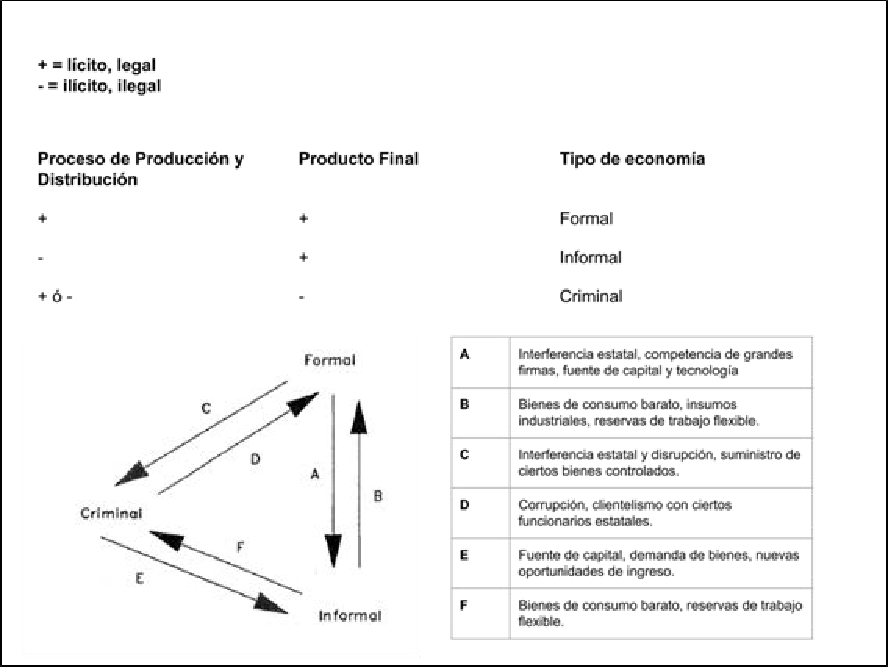
\includegraphics[width=5.20833in,height=\textheight]{Chapters/../Figures/portes_informal.pdf}

}

\end{figure}

\noindent \small Fuente: Portes et~al.
(\protect\hyperlink{ref-theinfo1989}{1989, p. 14}). Traducción propia
\normalsize

\hypertarget{causas-de-la-informalidad}{%
\section{Causas de la informalidad}\label{causas-de-la-informalidad}}

Existe debate acerca de las causas o al origen de la informalidad. Esto
ha llevado a que se generen corrientes que enfatizan cierto aspecto como
la causa principal que explica en mayor medida la informalidad.

\hypertarget{corriente-estructural}{%
\subsection{Corriente estructural}\label{corriente-estructural}}

La corriente estructuralista
(\protect\hyperlink{ref-acemoglu2001}{Acemoglu, 2001};
\protect\hyperlink{ref-cacciamali1983}{Cacciamali, 1983};
\protect\hyperlink{ref-souza1980}{Souza, 1980};
\protect\hyperlink{ref-tokman1978}{Tokman, 1978}), predominante en los
años 80, considera que la principal causa de la permanencia y aumento
del sector informal es debido a que existe un sector de la economía
``moderno'' en la que se concentran los ``buenos empleos'', las
innovaciones tecnológicas, inversiones de capital extranjero, mano de
obra calificada y alta productividad, y que mantiene al margen a un
sector de la economía ``tradicional'' en el que se encuentran los
``malos'' empleos, trabajadores poco calificados y pagados con baja
productividad. Esta aproximación dualista de la economía considera que
es insuficiente la demanda laboral en el sector formal de la economía
para absorber a la masa de trabajadores y proveer empleo sobre todo poco
calificados por lo que las pequeñas empresas y empresas familiares optan
por la informalidad como una alternativa de supervivencia. Desde esta
aproximación, el sector informal tiene un desenvolvimiento subordinado
al desarrollo del sector formal, y emerge como resultado de la falta de
oportunidades laborales y económicas en una región o país. La principal
causa se asocia a factores económicos, falta de desarrollo productivo.
Algo positivo de este enfoque es que plantea una interrelación entre el
sector formal y el sector informal, cuentan con vasos comunicantes y no
son compartimentos estancos.

No obstante, esta perspectiva ha sido criticada Carneiro
(\protect\hyperlink{ref-carneiro1997}{1997}) debido a que se ha podido
observar de que en zonas económicamente activas en donde hay creación de
empleo y fluidez de capital, el empleo informal crece con mayor rapidez
junto con el empleo formal. En un estudio realizado en Brasil, Carneiro
(\protect\hyperlink{ref-carneiro1997}{1997}) demostró como en las
regiones en donde había mayor dinamismo económico y el empleo formal
estaba creciendo, crecía también en mayor medida el empleo informal que
en otras regiones con menor crecimiento económico (p.~16). El autor
argumenta que este fenómeno podría deberse a la creciente importancia
del sector servicios, y una crisis de la regulación estatal, es decir,
la incapacidad del gobierno de intervenir en el sistema productivo.
Asimismo, Pinilla Cisneros
(\protect\hyperlink{ref-cosamaluxf3n2018}{Cosamalón, 2018}) afirma que
esta corriente no incorpora el papel del Estado como un actor decisivo
en la propagación del sector informal y tampoco consideraba la
subcontratación hacia el sector informal de las grandes empresas.

\hypertarget{corriente-neoliberal}{%
\subsection{Corriente neoliberal}\label{corriente-neoliberal}}

La corriente neoliberal (\protect\hyperlink{ref-beiner1989}{Beiner,
1989}; \protect\hyperlink{ref-belapatiuxf1o2017}{Belapatiño et~al.,
2017}; \protect\hyperlink{ref-cartaya1987}{Cartaya, 1987};
\protect\hyperlink{ref-desoto1987}{H. de Soto et~al., 1987}),
predominante en los años 90 junto con el auge político del
neoliberalismo, considera que la principal causa del sector informal es
la excesiva reglamentación estatal del mercado laboral y el costo de
transacción en las actividades económicas. De esta manera, la
legislación laboral directa o indirectamente desincentiva la
contratación formal en tanto que suelen ser rígidas y no permiten la
flexibilidad en la contratación y despido de personal para superar las
imperfecciones del mercado. Esto, sumado a la percepción de que no
representa ningún beneficio para la empresa tener trabajadores formales
vuelve poco atractivo el proceso de formalización, a falta de incentivos
fiscales, y genera a que se incurra y perdure en la informalidad. En
adición, H. de Soto et~al. (\protect\hyperlink{ref-desoto1987}{1987})
plantea que los engorrosos trámites burocráticos serían una barrera de
ingreso por los sectores acomodados para impedir que los trabajadores
pobres accedan a los beneficios sociales y servicios del Estado.

Esta corriente enfatiza que el sector informal no solo está conformado
por pequeños negocios, sino también medianos y grandes con alta
productividad, tecnología y salarios, pero que incurren en tener
trabajadores no registrados, autoempleados, trabajadores independientes
no cubiertos en el seguro social
(\protect\hyperlink{ref-belapatiuxf1o2017}{Belapatiño et~al., 2017}).

Un aspecto positivo de esta corriente es que permitió considerar, como
parte del sector informal, a las actividades legitimas llevadas a cabo
por compañías formales que por múltiples razones eligen mantener una
parte de sus operaciones en la informalidad con trabajadores no
registrados. Esto, más adelante, fue catalogado como ``empleo informal
en el sector formal'' (\protect\hyperlink{ref-inei2020}{INEI, 2020}).
Asimismo, recuperó el papel de la decisión de los actores que antes eran
entendidos como víctimas pasivas de causas estructurales y había poco
que podían hacer para escapar de la situación de informalidad.

No obstante, esta perspectiva ha sido criticada por distintos autores
(\protect\hyperlink{ref-cosamaluxf3n2018}{Cosamalón, 2018};
\protect\hyperlink{ref-theinfo1989}{Portes et~al., 1989}) dado que
romantiza el sector informal peruano, ensalzan la informalidad como
reafirmación del espíritu empresarial en América Latina y promueven el
camino informal como una solución generalizada a las crisis económicas
de los países en que el sector tiene gran influencia. En la medida en
que se concentran en el proceso de formalización y sus limitaciones, se
deja de lado o en segundo plano lo que significa ser ``formal'' en
términos de beneficios sociales y cobertura; lo cual, puede llegar a ser
una limitación al momento de plantear soluciones. Por otro lado, esta
corriente rara vez incluye en su análisis los factores estructurales
como el modelo de desarrollo o el desempeño macroeconómico de un país.
Asimismo, Cosamalón agrega que en muchas ocasiones, principalmente en
América Latina, la difusión del comercio informal respondió
principalmente a un repliegue del Estado y de sus medios de coacción por
crisis fiscal, alteración política, violencia insurgente, entre otras,
lo que permitió el surgimiento de actores que rivalizaran con las
autoridades sobre el control del espacio público como fue el caso de
Perú en los 80's (\protect\hyperlink{ref-cosamaluxf3n2018}{2018, p. 5}).

\hypertarget{corriente-multicausal}{%
\subsection{Corriente multicausal}\label{corriente-multicausal}}

Durand (\protect\hyperlink{ref-durand2007}{2007}) comenta que la
economía informal ``está constituida por empresas y trabajadores que
operan en una zona institucional claroscura''. Por lo que su nivel de
transgresión a la norma es limitado en tanto que no han cometido un
delito lesivo a la propiedad y a la persona. En el caso peruano, la
informalidad se suele reproducir cuando, por ejemplo, un conjunto de
ambulantes empieza a frecuentar una zona urbano-marginal para la venta
de sus bienes y servicios. Luego de generarse una masa crítica, se
constituyen los mercados informales en ``zonas liberadas'' del control
del Estado.

De esta manera, se reconoce el papel del Estado de reglar, fiscalizar
(enforcement) y de establecer los mecanismos hacia la formalidad, pero
que; sin embargo, con frecuencia carecen de la capacidad para regular
plenamente las actividades y derechos en las sociedades
(\protect\hyperlink{ref-cosamaluxf3n2018}{Cosamalón, 2018}). Si bien el
Estado conoce la ubicación de estos espacios informales (e.g el
principal local de Sunat se encuentra a 3 cuadras de varios centros
comerciales de softwares piratas), su intervención es esporádica o
muchas veces nulas dependiendo de múltiples causas como un desborde para
controlar la economía, coimas a los funcionarios, entre otros. Dentro
del régimen de la economía informal, los trabajadores no se encuentran
en una planilla, si algún derecho tienen, este se da por costumbre antes
que por ley (\protect\hyperlink{ref-durand2007}{Durand, 2007, p. 81}).

Asimismo, Céspedes Reynaga
(\protect\hyperlink{ref-cuxe9spedesreynaga2020}{2020}) argumenta que la
informalidad resulta en un mecanismo de suavización de la contracción
y/o expansión economía. Por ello, muchos trabajadores optarían por el
sector informal al ser menos costosos el riesgo de desempleo en épocas
de crecimiento económico.

\hypertarget{corriente-neoestructural}{%
\subsection{Corriente neoestructural}\label{corriente-neoestructural}}

Portes et~al. (\protect\hyperlink{ref-theinfo1989}{1989}) argumentan que
la informalidad laboral se debe principalmente a un proceso de
reestructuración económica mundial a raíz de la crisis del petróleo en
1973. A partir de este acontecimiento, las empresas internacionales,
para ser más competitivas, recurren en mayor medida al trabajo intensivo
informal por lo que no solo les beneficia la permanencia del sector
informal sino también su crecimiento y robustez. Estas empresas, muchas
veces en la forma de ``maquiladoras'', empresas financiadas por capital
extranjero para importar, procesar materia prima y exportarla a los
mismos países con valor agregado, buscan tercerizar su producción en el
sector informal abaratando costos. Esto se podría entender como un
proceso de descentralización productiva donde los sectores modernos
globales subcontratan para realizar sus actividades tanto a nivel
nacional como internacional, reificando y promoviendo que las pequeñas y
medianas empresas tengan trabajadores sin contrato laboral para reducir
costos y operar con las tarifas más bajas.

Por otro lado, plantean una caracterización de la informalidad que
incluya la amplitud de casos posibles en este sector. En primer lugar,
mencionan que la informalidad es un componente integrado en las
economías nacionales. No se desarrolla de manera independiente a la
economía formal, sino que interactúan para satisfacerse mutuamente
(\protect\hyperlink{ref-theinfo1989}{1989, p. 26}). En segundo lugar,
los trabajadores de la economía informal laboran en una condición
degradada en términos de beneficios sociales (seguro contra accidentes,
fondo de pensiones, entre otros). A la par, es más difícil establecerse
como un colectivo de presión (e.g un sindicato) dada la falta de
estabilidad en su labor sin contratos que lo aten. En tercer lugar, si
bien los trabajadores informales son muchas veces intervenidos por los
efectivos policiales, la actividad informal se desarrolla ampliamente
bajo la tolerancia del gobierno ya sea para evitar conflictos sociales o
para establecer patronaje político.

\hypertarget{efectos-de-la-informalidad}{%
\section{Efectos de la informalidad}\label{efectos-de-la-informalidad}}

A diferencia de las causas, existe relativo consenso acerca de las
consecuencias que puede traer el sector informal para la economía, las
empresas y los trabajadores. Con respecto a la economía, se forma un
modelo descentralizado de organización económica que busca reducir los
costos de producción (\protect\hyperlink{ref-theinfo1989}{Portes et~al.,
1989}). Las conexiones y subcontratación hacia el sector informal
generan un aumento de microempresas con múltiples proveedores que
contribuyen una fracción de la producción total.

Cabe mencionar que la informalidad representa de por sí una menor
recaudación de tributaria que representa un obstáculo para la provisión
de bienes y servicios públicos
(\protect\hyperlink{ref-belapatiuxf1o2017}{Belapatiño et~al., 2017}). El
impuesto a la renta no recaudado del sector informal podría haber sido
invertido en educación, salud, justicia, infraestructura, seguridad
ciudadana, entre otras. Este déficit en la recaudación de impuestos
resulta en una sobrecarga impositiva en el sector formal dado que se
trata de optimizar al máximo la recaudación en este sector y de esta
manera también se afecta la productividad y competitividad de las
actividades formales.

Con respecto a las empresas, la informalidad laboral reduce su
productividad en tanto que las condiciones precarias y el bajo
equipamiento con la que laburan sus trabajadores les impide rentabilizar
su productividad.

Con respecto a los trabajadores, se debilita el poder de lucha sindical
o la capacidad de exigir un cambio de los trabajadores que contribuyen
al sector informal dado que no existen mecanismos legales que garanticen
su permanencia en un oficio (\protect\hyperlink{ref-theinfo1989}{Portes
et~al., 1989}). En el sector informal abundan las relaciones de trabajo
inestables, temporales y esporádicas por lo que el trabajador informal
debe alinearse con las condiciones precarias de trabajo, los horarios
abusivos, entre otros, porque siempre existe la posibilidad de ser
reemplazado por un ejército de desempleados dispuesto a someterse a esas
condiciones de trabajo. Asimismo, la informalidad tiende a trasladar los
costos de la producción a los trabajadores siendo cada vez más común los
talleres domiciliarios sustituyendo a las fábricas centralizadas.

\hypertarget{salidas-a-la-informalidad}{%
\section{Salidas a la informalidad}\label{salidas-a-la-informalidad}}

Belapatiño et~al. (\protect\hyperlink{ref-belapatiuxf1o2017}{2017})
sugiere que se modifique la normativa laboral para promover la
formalización de las empresas en términos de flexibilizar las relaciones
laborales. Es así como manifiesta la necesidad de facilitar la
contratación y el despido en una empresa formal para que el negocio
pueda superar situaciones adversas o inesperadas en la economía y el
mercado laboral como lo es la pandemia del COVID-19. Esto se puede ver
reflejado en un estudio realizado por Apoyo Consultoría se muestra que
54\% de los empleadores entrevistados mencionó que su principal tema de
preocupación en materia laboral es la dificultad para despedir
trabajadores, 43\% comenta que es difícil gestionar los recursos humanos
en el marco de la fiscalización del Estado), 35\% resalta el
encarecimiento de mano de obra calificada.

Asimismo, se sugiere la simplificación de la reglamentación laboral para
reducir los trámites y el tiempo que toma para que una empresa formal se
pueda constituir (\protect\hyperlink{ref-belapatiuxf1o2017}{Belapatiño
et~al., 2017}). Inclusive plantear incentivos tributarios para que las
empresas registren a sus trabajadores y mantengan en regla sus archivos
contables.

Otra posibilidad que plantean diferentes autores
(\protect\hyperlink{ref-belapatiuxf1o2017}{Belapatiño et~al., 2017}) es
la implementación de salarios mínimos diferenciados por el sector
productivo en el cual se labore.

Existen salidas de la informalidad que hacen énfasis en mejorar la
productividad de los trabajadores a través de condiciones estructurales.
Céspedes Reynaga (\protect\hyperlink{ref-cuxe9spedesreynaga2020}{2020})
argumenta que, si bien el crecimiento económico y la productividad del
sector formal empuja la generación de empleo hacia la formalidad, el
efecto es mínimo por lo que se requiere de otras soluciones más
directas. Entre estas se podrían considerar políticas activas que
mejoren el nivel educativo, la calidad y cobertura de los servicios de
salud, la infraestructura vial, entre otros. Este aumento de la
productividad debe ser focalizado; ya que, no todos los sectores de la
economía operan al mismo nivel de productividad.

Según el INEI (\protect\hyperlink{ref-belapatiuxf1o2017}{Belapatiño
et~al., 2017}), el sector ``minero e hidrocarburos'' es 40 veces más
productivo que el ``agropecuario y pesca'', y el sector ``servicios y
comercio'', donde se ubica la mayor parte de la PEA ocupada, es 6 veces
más productivo que el ``agropecuario y pesca''. De esta manera, se
entiende que uno de los sectores en que es más urgente intervenir para
reducir la informalidad es el sector ``servicios y comercio'' por su
predominancia en la economía peruana. Ahora bien, Beteta
(\protect\hyperlink{ref-beteta2020}{2020}) afirma que en el 2019, en
América Latina, la mayoría de empleos nuevos se generaron en los
sectores de comercio de los restaurantes y hoteles caracterizado por la
concentración de empleo informal; sin embargo, fue justamente este
sector el cual fue el más impactado por la pandemia del COVID-19 que
dispuso a los gobiernos a aplicar cuarentenas parciales o totales, se
limitaron los aforos, el poder de compra de los trabajadores se estancó,
entre otras barreras que experimentaron estas empresas ya sea formales
como informales.

\hypertarget{caso-internacional}{%
\section{Caso internacional}\label{caso-internacional}}

La Organización Internacional del Trabajo entiende al ``sector
informal'' como el universo de establecimientos de las unidades de
producción dedicadas a la producción de bienes y/o servicios con la
finalidad de crear empleos y generar ingresos para las personas
involucradas en la actividad económica
(\protect\hyperlink{ref-oit2002}{OIT, 2002}). Las unidades de producción
en la economía informal presentan principalmente los rasgos de las
empresas de hogares, es decir, que las obligaciones de la empresa no
recaen en sí misma sino en sus propietarios, y es a nombre ellos que se
efectúan las transacciones con otras unidades productivas. Es por ello
por lo que, muchas veces, los gastos de la empresa se encuentran
indistinguibles de los gastos de las familias involucradas en la
producción. La OIT menciona que estas empresas de empleadores informales
se caracterizan por tener una baja cantidad de empleados, estos
empleados suelen no estar oficialmente registrados, entre otros.

Por otro lado, el ``empleo informal'' se entiende como el número total
de empleos informales de los trabajadores involucrados en la economía
(\protect\hyperlink{ref-oit2002}{OIT, 2002}). Dentro de esta categoría
se encuentran, por ejemplo, los trabajadores y empleadores por cuenta
propia (independientes) dueños de sus propias empresas del sector
informal, trabajadores familiares auxiliares ya sean partícipes del
sector formal e informal, miembros de cooperativas de productores
informales (no constituidas formalmente ante entidades legales),
asalariados (no sujetos a la legislación laboral nacional) que tienen
empleos informales, entre otros.

\hypertarget{caso-peruano}{%
\section{Caso peruano}\label{caso-peruano}}

Un exponente peruano de los estudios sobre el sector informal es
Hernando de Soto, quien fue un autor influyente, principalmente en los
90's, llegando a tener un impacto directo en diferentes políticas
públicas. Un ejemplo de ello es el Comisión de Formalización de la
Propiedad Informal (COFOPRI). De H. de Soto et~al.
(\protect\hyperlink{ref-desoto1987}{1987}) consideraba que los elevados
costos de la formalidad llevaban a al auge de la construcción informal y
por consecuencia a las barriadas, las cuales eran vistas como un proceso
autogestionario frente a la ineficiencia estatal. De esta manera,
resultaba lógico que si el Estado reconocía la formalidad del terreno
ocupado de manera informal podía tener una influencia positiva en el
tipo de actividades laborales que se realizaban en estos espacios
mientras que se recaudaban impuestos de estos terrenos a la par que los
autoempleados se convertían propietarios de sus medios de producción
abalados por el Estado y así superar la pobreza urbana. De esta manera,
en el marco de la política de la titulación masiva por parte del
gobierno fujimorista se crea COFOPRI en 1996, con asesoría de H. de Soto
y el financiamiento del Banco Mundial. Sin embargo, en la práctica este
organismo se dedicó únicamente a la entrega de títulos de dominio y no
se reparó en la calidad de la vivienda y del espacio en que se construía
(\protect\hyperlink{ref-torres2019}{Torres \& Ruiz-Tagle, 2019}).

Esquivel (\protect\hyperlink{ref-esquivel2011}{2011}) argumenta que en
términos de entregar títulos de propiedad la comisión fue efectiva; pero
que, si observamos los objetivos que realmente buscaba cambiar damos
cuenta con que la inversión realizada en la propiedad posterior a la
entrega fue mínima, el acceso a servicios básicos fue reducido, la
obtención de préstamos bancarios fue principalmente estatal y rara vez
de entidades privadas, entre otros
(\protect\hyperlink{ref-esquivel2011}{2011, p. 2}). Asimismo, la
política pública de formalización urbana con COFOPRI ha traído como
consecuencia el incremento de tráfico de terrenos dada la simplicidad de
trámites en la obtención de títulos de dominio inclusive desconociendo a
dueños anteriores. De esta manera, resultó insuficiente la explicación
de que la informalidad se debía principalmente a la falta de extensión
del crédito y las hipotecas dado que en la práctica requería mucho más
que eso.

Ahora bien, en concordancia con las directrices planteadas por la OIT,
el Instituto Nacional de Estadística e Informática (INEI, Perú) ha
adoptado como parte del estudio y monitoreo de la economía informal la
dualidad entre el sector y el empleo informales.

El primero, según el INEI, refiere a las ``empresas de hogares (unidades
productivas no constituidas en sociedad, excluyendo las cuasisociedades)
que no están registradas en la administración tributaria (SUNAT)''
(\protect\hyperlink{ref-inei2020}{INEI, 2020}).

En tanto que la unidad de estudio son las unidades productivas, se busca
recopilar esta información a través de una ``Encuesta de
establecimientos'' principalmente. El segundo, se encuentra enmarcado en
el total de empleos que cumplen con alguna de las siguientes
condiciones: a) los patronos y cuenta propia cuya unidad productiva
pertenece al sector informal, b) asalariados sin seguridad social
financiada por su empleador, c) los trabajadores familiares no
remunerados que laboran la unidad productiva. En tanto que la unidad de
estudio son las unidades productivas, se busca recopilar esta
información a través de una ``Encuesta de establecimientos''
principalmente. Esta distinción nos permite apreciar los empleos
informales que se encuentran fuera del sector informal considerando a
aquellos asalariados del sector ``formal'' con empleo informal.

\begin{figure}

\caption{\label{fig-pea}Clasificación de la PEA informal}

{\centering 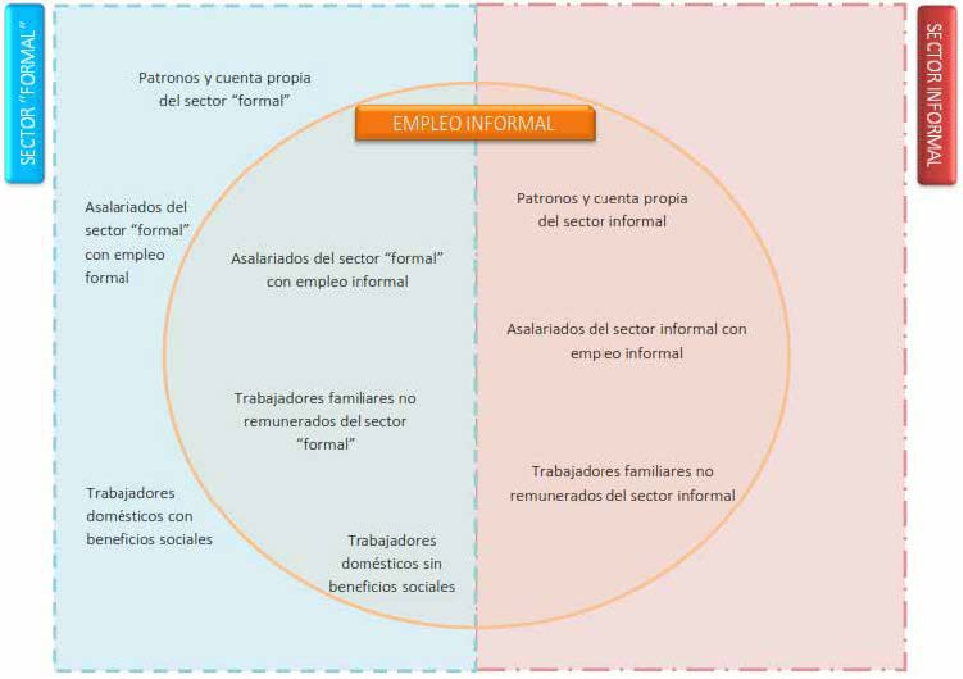
\includegraphics[width=5.20833in,height=\textheight]{Chapters/../Figures/pea_informal1.pdf}

}

\end{figure}

\noindent \small Fuente: Instituto Nacional de Estadística e Informática
-- 2017: ``Producción y Empleo Informal en el Perú 2017-2016''; en
Mantilla (\protect\hyperlink{ref-mantilla2021}{2021}) \normalsize

Cosamalón (\protect\hyperlink{ref-cosamaluxf3n2018}{2018}) destaca,
desde una aproximación cualitativa la informalidad en el Perú, de que
una de las figuras centrales en el sector informal es el vendedor
ambulatorio que no solo vende un stock de productos en la calle para
poder sobrevivir, sino que es parte de un proceso de reconfiguración de
la economía mundial.

Sobre el caso peruano, Cosamalón tiene especial interés en las formas de
supervivencia que se utilizaron en las calles, a lo que comúnmente se
denomina ``trabajo callejero'' pero sin desmerecer la memoria y dignidad
de las personas que buscan salir adelante por sus propios medios. La
figura del vendedor ambulante se encuentra bastante presente en el Perú
donde la disminución del salario real, en la década de 1990, deprimió la
capacidad de consumo de los diferentes estratos sociales creando una
demanda por el precio más bajo. Plantea, además, que resulta crucial el
rol del ``capital social'' para comprender las dinámicas del sector
informal urbano y en especial al fenómeno ambulatorio. Como hemos
mencionado anteriormente, al no contar con mecanismos de protección
social públicos, los trabajadores informales crean sus propias redes de
apoyo mutuo las cuales requieren inversión y mantenimiento.

Estudios realizados en nuestro país
(\protect\hyperlink{ref-cuxe9spedesreynaga2020}{Céspedes Reynaga, 2020};
\protect\hyperlink{ref-chacaltana2016}{Chacaltana, 2016}) destacan lo
siguiente utilizando bases de datos como la Encuesta Nacional de Hogares
(ENAHO) y la Encuesta Permanente de Empleo (EPE). En primer lugar, la
informalidad urbana promedio varía entre 53\% y 75\% dependiendo de la
definición operativa que se utilice y sin considerar tiempos de crisis.
En segundo lugar, la informalidad laboral entre 2004 y 2014 se redujo
entre -2,4\% y -0.5\%. Esta reducción ha venido a la par con un
incremento de la tasa de empleo formal principalmente entre los
trabajadores asalariados que entre 2002 y 2012 pasó del 41\% al 50\%
(\protect\hyperlink{ref-chacaltana2016}{Chacaltana, 2016, p. 52}).

Rodríguez \& Higa (\protect\hyperlink{ref-rodruxedguez2010}{2010})
confirman, utilizando la ENAHO, que el denominado ``sector informal'' ha
tenido una lenta tendencia a la baja independientemente que definición
se utilice en la década del 2000, lo cual se verá que difiere de la
situación actual. Asimismo, muestran que la conducción de las unidades
de producción informales suele estar a cargo de las mujeres. Esta
tendencia ha ido en aumento constituyéndose en un 56,2\% de mujeres en
el 2008 (p.19). Por otro lado, en relación con las unidades productivas,
observan que el 55\% no cuentan con local fijo, entre 10\% y 20\%
cuentan con servicios de agua y desagüe en su local, aunque poco más de
la mitad cuenta con electricidad en su local de trabajo, cerca del 3\%
cuenta con telefonía o internet.

Más aún, Higa et~al. (\protect\hyperlink{ref-higa2021}{2021}) señala que
durante el primer año de la pandemia, los más afectados dentro de la
fuerza laboral fueron los trabajadores poco calificados, los
trabajadores de servicios, los jóvenes, mujeres (sobre todo con hijos
menores), y minorías étnicas. Asimismo, se ha incrementado la brecha
entre los trabajadores con educación y los que cuentan con menor
educación formal. Esta brecha se incrementó al inicio de la pandemia y
ha persistido más de un año después. Este estudio publicado en 2021 se
cuestiona si la brecha será superada una vez la pandemia esté bajo
control.

Si consideramos las principales características estructurales de la
informalidad laboral en el Perú, distintos autores
(\protect\hyperlink{ref-barco2010}{Barco \& Vargas, 2010};
\protect\hyperlink{ref-cuxe9spedesreynaga2020}{Céspedes Reynaga, 2020};
\protect\hyperlink{ref-chacaltana2016}{Chacaltana, 2016};
\protect\hyperlink{ref-rodruxedguez2010}{Rodríguez \& Higa, 2010})
mencionan las siguientes:

\begin{itemize}
\item
  La informalidad laboral usualmente cuenta con trabajadores con pocos
  años de educación.
\item
  Cuenta con trabajadores con pocas habilidades laborales.
\item
  Cuenta con trabajadores con bajo nivel educativo.
\item
  Laboran en micro y pequeñas empresas.
\item
  Afecta mayormente a las mujeres.
\item
  Afecta mayormente a los empleos no asalariados.
\item
  Afecta principalmente a trabajadores jóvenes y adultos mayores.
\item
  Es mayor en áreas urbanas fuera de Lima Metropolitana.
\item
  Predomina en el sector de comercio, construcción y en actividades
  primarias.
\end{itemize}

Hemos visto que no existe una definición conceptual singular de la
informalidad laboral, en parte, por el distinto énfasis que se le otorga
a la diversos elementos que constituyen la informalidad. Del mismo modo,
Céspedes Reynaga (\protect\hyperlink{ref-cuxe9spedesreynaga2020}{2020})
considera que existen múltiples definiciones operativas al momento de
querer medir el fenómeno en cuestión, para identificar a los
trabajadores informales en una economía.

El INEI identifica a los trabajadores informales considerando la
diferencia entre el sector informal y el sector formal establecido por
la OIT en su XIII Conferencia Internacional de Estadísticas de Trabajo o
CIET por sus iniciales
(\protect\hyperlink{ref-cuxe9spedesreynaga2020}{Céspedes Reynaga,
2020}). Asimismo,

\begin{quote}
``considera como trabajador informal a los patronos y por cuenta propia
cuya unidad productiva pertenece al sector informal, los asalariados
(del sector formal) sin seguridad social financiada por su empleador, y
los trabajadores familiares no remunerados, independientemente de la
naturaleza formal o informal de la unidad productiva donde trabaja''
(Céspedes Reynaga, 2020).
\end{quote}

Céspedes Reynaga afirma que, para cubrir los diferentes casos, se
plantean los siguientes tipos de definiciones operacionales para
identificar trabajadores informales dependientes asalariados y para los
trabajadores del hogar:

\begin{itemize}
\item
  Informalidad por ingresos: incluye a los trabajadores informales que
  perciben un salario mínimo por hora menor al establecido por la ley
  (actualmente s/.1025).
\item
  Informalidad por afiliación al sistema de pensiones: incluye a los
  trabajadores informales que declaran no estar afiliados a ningún
  sistema de pensiones (público o privado).
\item
  Informalidad por libros contables: incluye a los trabajadores
  informales que mencionaron conocer que la empresa donde labora no
  lleva libros contables.
\item
  Informalidad por personería jurídica: trabajadores informales que
  trabajan en empresas sin personería jurídica.
\item
  Informalidad por contrato: trabajadores informales que laboran sin
  ningún tipo de contrato.
\item
  Informalidad por impuestos laborales: trabajadores informales que
  mencionaron no pagar ningún descuento laboral.
\end{itemize}

Considerar los distintos tipos de informalidad de manera independiente y
en su conjunto es útil cuando no se cuenta con información acerca de
alguno de los indicadores.

\hypertarget{suxedntesis}{%
\section{Síntesis}\label{suxedntesis}}

Luego de lo expuesto, podemos concluir que siendo la informalidad
laboral una temática desarrollada a finales del siglo pasado, una gran
cantidad de estudios se limitan a estudiarla como un todo unificado
(cantidad de personas involucradas, producción económica anual, etc.) y
no predominan los estudios que se concentren en la diferenciación y
variedad de casos que existen dentro de la informalidad. Este es un
vacío que la presente investigación busca compensar.

\bookmarksetup{startatroot}

\hypertarget{sec-marco}{%
\chapter{Marco Teórico}\label{sec-marco}}

Para este estudio, me basaré en las definiciones planteadas por el INEI,
que a su vez se apoyan en los lineamientos sugeridos por la OIT, en
tanto que utilizo como fuente de información las bases de datos
recopiladas en la Encuesta Nacional de Hogares (ENAHO). En adición, se
acota la población de estudio a los trabajadores ubicados en las urbes
del Perú dado que la experiencia de la informalidad laboral difiere
tanto en el ámbito rural como en el urbano, lo cual tiene implicancias
en el estudio de las condiciones de vida.

Para identificar a los trabajadores informales, el INEI selecciona a la
Población en Edad de Trabajar (PET) la cual consiste en las personas de
14 años a más y que, a su vez, se subdivide en Población Económicamente
Activa (PEA) y Población Económica Inactiva (PEI). La primera, refiere a
aquellos que en la semana de referencia consultada en la encuesta se
encontraban trabajando, no trabajaban, pero tenían trabajo, o se
encontraban buscando activamente un trabajo. La segunda, refiere a
aquellos que no se encontraban buscando un trabajo a la fecha. Dentro de
la PEA, se considera como ``ocupados'' a todos aquellos que estuvieron
participando en alguna actividad económica; los trabajadores
dependientes que aunque tuvieron un empleo fijo no trabajaron la semana
anterior por motivo de vacaciones, huelga, licencia por enfermedad,
licencia de maternidad, entre otras, todas estas pagadas; los
trabajadores independientes que estuvieron ausentes en sus trabajos pero
la empresa o negocio continúa funcionando; los trabajadores que no
teniendo un empleo constante realizaron un oficio por al menos una hora
y fueron remunerados con dinero y/o especie; por último, los
trabajadores familiares no remunerados que trabajaron 25 horas o más,
practicantes, fuerzas armadas y policiales.

Como hemos visto anteriormente, el estudio de la informalidad se puede
abordar desde el punto de vista de las unidades productivas fuera de los
registros públicos (sector informal) o de la fuerza laboral (empleo
informal) la cual puede trabajar sin un contrato formal, sin beneficios
sociales, en condiciones de trabajo deplorables, entre otras. En la
medida en que nos centraremos en estudiar las condiciones de vida,
representadas en el ingreso mensual, optaremos por centrarnos en el
``empleo informal'' y en el ``empleo formal''.

\hypertarget{empleo-informal}{%
\section{Empleo informal}\label{empleo-informal}}

El empleo informal refiere al total de empleos dentro de la Población
Económicamente Activa Ocupada (PEAO) que cumplen alguna de las
siguientes condiciones, según la categoría de ocupación del trabajador:

\begin{enumerate}
\def\labelenumi{\roman{enumi})}
\tightlist
\item
  Los patronos y cuenta propia cuya unidad productiva pertenece al
  sector informal.
\item
  Los asalariados sin seguridad social financiada por su empleador.
\item
  Los trabajadores familiares no remunerados, independientemente de la
  naturaleza formal o informal de la unidad productiva donde labora.
\end{enumerate}

Dentro del empleo informal se puede distinguir entre dos grupos siendo
los que trabajan de manera independiente, y los que se desenvuelven
dentro unidades productivas: empleados, empleadores, obreros y
trabajadores familiares no remunerados
(\protect\hyperlink{ref-cuxe9spedesreynaga2020}{Céspedes Reynaga, 2020};
\protect\hyperlink{ref-sanchuxe9zvillagomez2019}{Sanchéz Villagomez \&
Chafloque Céspedes, 2019}). Asimismo, como hemos mencionados
anteriormente, la barrera entre el sector formal y el informal es
porosa, y fluctúan los empleos informales entre ambos sectores con
condiciones laborales muy distintas; no obstante, predominan las
condiciones precarias.

\hypertarget{empleo-formal}{%
\section{Empleo formal}\label{empleo-formal}}

Comprende a los patronos y cuenta propia, asalariados y trabajadores
domésticos con beneficios sociales del sector formal
(\protect\hyperlink{ref-inei2021}{INEI, 2021}).

\hypertarget{condiciones-de-vida}{%
\section{Condiciones de vida}\label{condiciones-de-vida}}

Entenderemos como ``condiciones de vida'' al ingreso neto que tienen los
hogares que les permiten satisfacer sus necesidades a través de bienes
de consumo y servicios. Con el objetivo de observar el impacto directo
de la pandemia en las condiciones de vida de los trabajadores y sus
hogares, se ha priorizado como indicador el ingreso mensual proveniente
del trabajo. De esta manera, se considera el ingreso promedio
correspondiente a la PEA ocupada con ingresos mayores a cero y que
provienen de su actividad principal, secundaria, trabajo dependiente e
independiente, y puede llegar a ser monetario o no monetario (pago en
especias). Asimismo, se procesa esta variable para los residentes
habituales, ya sean miembros del hogar o no miembros, pero que
estuvieron presentes en el hogar en los últimos 30 días.

\hypertarget{nivel-de-pobreza}{%
\section{Nivel de pobreza}\label{nivel-de-pobreza}}

En 2010, la Comisión Consultiva para la Estimación de la Pobreza
(\protect\hyperlink{ref-inei2010}{INEI, 2010}) por encargo del INEI
mencionó, en función de los precios de la canasta de alimentos y la
remuneración mínima vital (RMV), que se podría definir los hogares
pobres cuyos ingresos se encuentran alrededor de s/.178 y s/.385. Este
cálculo ha sido establecido, a su vez, considerando la comparabilidad
con encuestas de años anteriores.

\bookmarksetup{startatroot}

\hypertarget{references}{%
\chapter*{References}\label{references}}
\addcontentsline{toc}{chapter}{References}

\markboth{References}{References}

\hypertarget{refs}{}
\begin{CSLReferences}{1}{0}
\leavevmode\vadjust pre{\hypertarget{ref-acemoglu2001}{}}%
Acemoglu, D. (2001). Good jobs versus bad jobs. \emph{Chicago},
\emph{vol.19}(N°1).

\leavevmode\vadjust pre{\hypertarget{ref-alonso1990}{}}%
Alonso, J. A. (1990). Review of The Informal Economy. Studies in
Advanced and Less Developed Countries. \emph{Estudios Sociológicos},
\emph{8}(22), 191-197. \url{http://www.jstor.org/stable/40420059}

\leavevmode\vadjust pre{\hypertarget{ref-barco2010}{}}%
Barco, D., \& Vargas, P. (2010). \emph{DT 2010 04: El Perfil del
Trabajador Informal y el Retorno de la Educación}.
\url{https://www.bcrp.gob.pe/publicaciones/documentos-de-trabajo/dt-2010-04.html}

\leavevmode\vadjust pre{\hypertarget{ref-beiner1989}{}}%
Beiner, B. (1989). \emph{A Economia Invis{ı}vel {\textemdash} Um
Survey}.

\leavevmode\vadjust pre{\hypertarget{ref-belapatiuxf1o2017}{}}%
Belapatiño, V., Grippa, F., \& Perea, H. (2017). \emph{Perú \textbar{}
Informalidad laboral y algunas propuestas para reducirla}. 21.

\leavevmode\vadjust pre{\hypertarget{ref-beteta2020}{}}%
Beteta, H. E. (2020). ¿Cómo encontró la pandemia del Covid-19 a América
Latina? / How did you find the Covid-19 pandemic in Latin America?
\emph{EconomíaUNAM}, \emph{17}(51), 180-193.
\url{https://doi.org/10.22201/fe.24488143e.2020.51.556}

\leavevmode\vadjust pre{\hypertarget{ref-cacciamali1983}{}}%
Cacciamali, M. C. (1983). \emph{Setor Informal Urbano e Formas de
Participaçao}. \emph{N. 20}.

\leavevmode\vadjust pre{\hypertarget{ref-carneiro1997}{}}%
Carneiro, F. (1997). The Changing Informal Labour Market in Brazil:
Cyclicality versus Excessive Intervention. \emph{LABOUR}, \emph{11}(1),
3-22. \url{https://doi.org/10.1111/1467-9914.00027}

\leavevmode\vadjust pre{\hypertarget{ref-cartaya1987}{}}%
Cartaya, V. (1987). El Confuso Mundo del Sector Informal.
\emph{Jul/Ago}, \emph{N. 90}.

\leavevmode\vadjust pre{\hypertarget{ref-cuxe9spedesreynaga2020}{}}%
Céspedes Reynaga, N. (2020). \emph{Crecer no es suficiente para reducir
la informalidad}. Universidad de San Martín de Porres.
\url{https://repositorio.usmp.edu.pe/handle/20.500.12727/8844}

\leavevmode\vadjust pre{\hypertarget{ref-chacaltana2016}{}}%
Chacaltana, J. (2016). \emph{Perú, 2002-2012: crecimiento, cambio
estructural y formalización}. CEPAL.
\url{https://www.cepal.org/es/publicaciones/40402-peru-2002-2012-crecimiento-cambio-estructural-formalizacion}

\leavevmode\vadjust pre{\hypertarget{ref-cosamaluxf3n2018}{}}%
Cosamalón, J. (2018). \emph{El apocalipsis a la vuelta de la esquina}.
Fondo Editorial, PUCP.

\leavevmode\vadjust pre{\hypertarget{ref-durand2007}{}}%
Durand, F. (2007). \emph{3. Las tres economías}. Fondo Editorial del
Congreso del Perú.

\leavevmode\vadjust pre{\hypertarget{ref-elcomercio2021}{}}%
El Comercio. (2021). Recuperación de la producción e informalización del
empleo, por Miguel Jaramillo \textbar{} Opinión \textbar{} ECONOMIA.
\emph{El Comercio Perú}.
\url{https://elcomercio.pe/economia/peru/recuperacion-de-la-produccion-e-informalizacion-del-empleo-por-miguel-jaramillo-opinion-noticia/}

\leavevmode\vadjust pre{\hypertarget{ref-esquivel2011}{}}%
Esquivel, A. (2011). \emph{Cofopri ¿organismo diseñado para mejorar el
bienestar de las personas?}
\url{http://repositorio.flacsoandes.edu.ec/handle/10469/2842}

\leavevmode\vadjust pre{\hypertarget{ref-hart1971}{}}%
Hart, K. (1971). Informal Income Opportunities and Urban Employment in
Ghana. \emph{unpublished}.

\leavevmode\vadjust pre{\hypertarget{ref-higa2021}{}}%
Higa, M., Ospino, C., \& Aragon, F. (2021). \emph{The persistent effects
of COVID-19 on labor outcomes: evidence from Peru}.
\url{https://ideas.repec.org/p/sfu/sfudps/dp21-10.html}

\leavevmode\vadjust pre{\hypertarget{ref-inei2010}{}}%
INEI. (2010). \emph{Evolución de la Pobreza al 2010}.

\leavevmode\vadjust pre{\hypertarget{ref-inei2020}{}}%
INEI. (2020). \emph{PERÚ: Evolución de los Indicadores de Empleo e
Ingreso por Departamento, 2007-2019}.

\leavevmode\vadjust pre{\hypertarget{ref-inei2021}{}}%
INEI. (2021). \emph{Perú: Evolución de los Indicadores de Empleo e
Ingreso por departamento, 2007-2020}.

\leavevmode\vadjust pre{\hypertarget{ref-ipe2020}{}}%
IPE. (2020). \emph{Mercado laboral peruano: impacto por covid-19 y
recomendaciones de política}.

\leavevmode\vadjust pre{\hypertarget{ref-loayza2020}{}}%
Loayza, N. V. (2020). \emph{Informalidad y crecimiento económico: Una
aproximación conceptual y una aplicación al Perú}. Universidad de San
Martín de Porres.
\url{https://repositorio.usmp.edu.pe/handle/20.500.12727/8843}

\leavevmode\vadjust pre{\hypertarget{ref-mantilla2021}{}}%
Mantilla, E. (2021). \emph{¿Y qué será de la vida?: un análisis de las
diferentes dimensiones de la vulnerabilidad a la pobreza de los hogares
peruanos, 2014-19}.

\leavevmode\vadjust pre{\hypertarget{ref-oecd2004}{}}%
OECD. (2004). \emph{Informal Employment and Promoting the Transition to
a Salaried Economy} (pp. 225-289).
\url{https://doi.org/10.1787/empl_outlook-2004-7-en}

\leavevmode\vadjust pre{\hypertarget{ref-oit2002}{}}%
OIT. (2002). \emph{Report VI: Decent work and informal economy}.

\leavevmode\vadjust pre{\hypertarget{ref-oit2021}{}}%
OIT. (2021). \emph{Transition from the informal to the formal economy -
Theory of Change}.
\url{https://www.ilo.org/wcmsp5/groups/public/---ed_protect/---protrav/---travail/documents/briefingnote/wcms_768807.pdf}

\leavevmode\vadjust pre{\hypertarget{ref-piore1987}{}}%
Piore, M. J., \& Sabel, C. F. (1987). The Second Industrial Divide.
\emph{Journal of Peace Research}, \emph{24}(2), 354 pp.
\url{https://doi.org/10.1177/002234338702400213}

\leavevmode\vadjust pre{\hypertarget{ref-theinfo1989}{}}%
Portes, A., Castells, M., \& Benton, L. A. (Eds.). (1989). \emph{The
Informal economy: studies in advanced and less developed countries}.
Johns Hopkins University Press.

\leavevmode\vadjust pre{\hypertarget{ref-rodruxedguez2010}{}}%
Rodríguez, J., \& Higa, M. (2010). Informalidad, empleo y productividad
en el Perú. \emph{Departamento de Economía}, \emph{Documento de Trabajo
282}.

\leavevmode\vadjust pre{\hypertarget{ref-sanchuxe9zvillagomez2019}{}}%
Sanchéz Villagomez, M., \& Chafloque Céspedes, M. R. (2019). \emph{La
informalidad laboral en el Perú: un mapa nacional basado en ENAHO}.
Universidad San Martín de Porres.
\url{https://www.administracion.usmp.edu.pe/investigacion/files/INFORMALIDAD-LABORAL-final-corregido.pdf}

\leavevmode\vadjust pre{\hypertarget{ref-desoto1987}{}}%
Soto, H. de, Ghersi, E., \& Ghibellini, M. (1987). \emph{El otro
sendero}. \url{https://books.google.com.pe/books?id=ZU95PQAACAAJ}

\leavevmode\vadjust pre{\hypertarget{ref-soto2020}{}}%
Soto, R. M., Cuéllar, N. G., \& Reyes-Olivo, M. (2020). Empleo y derecho
laboral en tiempos de pandemia, Perú 2020. \emph{Ciencia Latina Revista
Científica Multidisciplinar}, \emph{4}(2), 1497-1509.
\url{https://doi.org/10.37811/cl_rcm.v4i2.156}

\leavevmode\vadjust pre{\hypertarget{ref-souza1980}{}}%
Souza, P. R. (1980). Emprego, Salários e Pobreza. \emph{Hucitec,
Brazil}.

\leavevmode\vadjust pre{\hypertarget{ref-tokman1978}{}}%
Tokman, V. (1978). \emph{Las Relaciones entre los Sectores Formal e
Informal: Una Exploraci´on sobre su Natureza}. \emph{N. 5}.

\leavevmode\vadjust pre{\hypertarget{ref-torres2019}{}}%
Torres, D., \& Ruiz-Tagle, J. (2019). ¿Derecho a la vivienda o la
propiedad privada? De la política pública a la informalidad urbana en el
Área Metropolitana de Lima (1996-2015). \emph{136}, 5-29.

\leavevmode\vadjust pre{\hypertarget{ref-waldinger1985}{}}%
Waldinger, R., Ward, R., \& Aldrich, H. (1985). Ethnic Business and
Occupational Mobility in Advanced Societies. \emph{Sociology},
\emph{19}(4), 586-597. \url{https://doi.org/10.1177/0038038585019004007}

\end{CSLReferences}



\end{document}
